\documentclass[final]{thesis}
\usepackage[utf8]{vietnam}
\usepackage{placeins}
\usepackage{amsfonts}
\usepackage{textcomp}
\usepackage{dblfloatfix}
\usepackage{subfig}
\usepackage{lineno}
\usepackage{amssymb}
\usepackage{amsmath}
\usepackage{mathtools}
\usepackage{graphicx}
\usepackage{lscape}
\usepackage{caption}
\usepackage{hyperref}
\usepackage[sorting=ynt]{biblatex}
\usepackage{mathtools}
\usepackage{lipsum}
\usepackage{fancyhdr}
\usepackage{amsmath}
\usepackage{makecell}

% Config reference
\addbibresource{references.bib}

% Setup hype link in thesis
\hypersetup{urlcolor=blue,linkcolor=black,citecolor=black,colorlinks=true} 
\DeclarePairedDelimiter\bra{\langle}{\rvert}
\DeclarePairedDelimiter\ket{\lvert}{\rangle}
\DeclarePairedDelimiterX\braket[2]{\langle}{\rangle}{#1 \delimsize\vert #2}


% Config information thesis
\upperuniname{ĐẠI HỌC QUỐC GIA THÀNH PHỐ HỒ CHÍ MINH}
\uniname{TRƯỜNG ĐẠI HỌC CÔNG NGHỆ THÔNG TIN}
\deptname{KHOA MẠNG MÁY TÍNH VÀ TRUYỀN THÔNG}
\stumajor{KỸ SƯ NGÀNH AN TOÀN THÔNG TIN}
\title{CÁC KỸ THUẬT ẨN GIẤU THÔNG TIN TRONG ỨNG DỤNG VÀ DỮ LIỆU}
\titleen{Machine learning for pentest}
\supervisor{GIẢNG VIÊN HƯỚNG DẪN}
\supervisorname{TS. NGUYỄN NGỌC TỰ}
\stuname{TÔ TRỌNG NGHĨA \\NGUYỄN HỒNG SƠN \\ PHẠM TRẦN TIẾN ĐẠT \\ TẠ VIỆT HOÀNG }
\stunamewithid{NGUYỄN HỒNG SƠN - 220202022\\TÔ TRỌNG NGHĨA - 220202019 \\ PHẠM TRẦN TIẾN ĐẠT - 220202017 \\ TẠ VIỆT HOÀNG - 220202018}
\reporttime{NĂM 2023}

% Begin thesis
\begin{document}

\coverpage%
\secondcoverpage%

% % Begin above main thesis
\frontmatter
% \chapter*{\centering\Large{Thông tin hội đồng chấm khóa luận tốt nghiệp}}
\addcontentsline{toc}{chapter}{Thông tin hội đồng chấm khóa luận tốt nghiệp}
Hội đồng chấm khóa luận tốt nghiệp, thành lập theo Quyết định số 463/QĐĐHCNTT ngày 23 tháng 7 năm 2021 của Hiệu trưởng Trường Đại học Công nghệ
Thông tin.
\begin{center}
    \begin{tabular}{ p{.4\textwidth} p{.3\textwidth}} 
        1. TS. Nguyễn Tuấn Nam  & Chủ tịch \\
        2. ThS. Nguyễn Duy   & Ủy viên \\ 
        3. ThS. Trần Hồng Nghi & Thư ký \\ 
    \end{tabular} 
\end{center}



% \chapter*{\centering\Large{Lời cảm ơn}}
\addcontentsline{toc}{chapter}{Lời cảm ơn}
Không ai đạt được điều gì đó to lớn mà không nhờ sự giúp đỡ của những
người xung quanh, cho dù là trực tiếp hay gián tiếp đi nữa. Để hoàn thành được
khóa luận này, nhóm tác giả may mắn nhận được nhiều sự giúp đỡ và hỗ trợ từ
quý thầy, cô, anh chị, bạn bè và người thân. Nhóm tác giả xin dành những trang
đầu tiên này để bày tỏ lòng tri ân của mình tới tất cả mọi người, những người đã
đồng hành cùng nhóm trong khoảng thời gian vừa qua. \\
\indent Đầu tiên, nhóm tác giả xin gửi lời cảm ơn sâu sắc đến toàn thể các thầy cô
của Trường Đại học Công nghệ Thông tin nói chung và các thầy cô khoa Mạng
máy tính và Truyền thông nói riêng. Nhờ những kiến thức quý giá mà thầy cô đã
truyền đạt, cũng như việc hỗ trợ tận tình trong suốt khoảng thời gian thực hiện,
nhóm đã hoàn thành khóa luận và đạt được các kết quả đáng ghi nhận.
Nhóm tác giả xin đặc biệt cảm ơn TS. Nguyễn Ngọc Tự là người đã truyền
cảm hứng, tận tình hướng dẫn và hỗ trợ tận tình về kiến thức, tạo môi trường thuận
lợi để nhóm có thể học hỏi, trao đổi với các bạn, các em trong nhóm nghiên cứu.
Đây là những kiến thức, kinh nghiệm quý giá, không chỉ có tác dụng trong khóa
luận tốt nghiệp này mà còn trong khoảng thời gian làm việc trong chặng đường
tiếp theo. \\
\indent Trong giai đoạn dịch bệnh khó khăn, tình hình ngày càng phức tạp, dù có
khó khăn trong nhiều công việc, nhóm nhận được nhiều sự giúp đỡ và động viên
từ thầy cô và bạn bè. Đây là động lực to lớn thúc đẩy nhóm làm việc trong suốt
quá trình tìm hiểu và hoàn thành khóa luận này. \\
\indent Cuối cùng, nhóm tác giả không quên bày tỏ lòng tri ân đến gia đình và người
thân, những người đã luôn là những hậu phương vững chắc và luôn ủng hộ từng
quyết định mà nhóm đưa ra. \\
\indent Mặc dù đã nỗ lực rất nhiều để luận văn được hoàn thiện nhất, song khó có
thể tránh khỏi thiếu sót và hạn chế. Kính mong nhận được sự thông cảm và ý kiến
đóng góp từ quý thầy cô và các bạn.\\

\begin{flushright}
\textit {TP. Hồ Chí Minh, ngày 12 tháng 7 năm 2021} \\
\textit {Nhóm tác giả}
\end{flushright}


\tableofcontents
\clearpage
\listoffigures

\clearpage

\listoftables

% \chapter*{\centering\Large{Danh sách từ viết tắt}}
\addcontentsline{toc}{chapter}{Danh sách từ viết tắt}

\begin{tabular}{| p{.4\textwidth} |p{.4\textwidth} |}

        \hline
        RL &  \textbf{R}einforcement \textbf{L}earning        \\
        \hline
        MDP &  \textbf{M}arkov \textbf{D}ecision \textbf{P}rocesses     \\
        \hline
\end{tabular} \\



\clearpage

% Begin main thesis, start page numbering
\counterwithin{equation}{chapter}
\counterwithin{table}{chapter}
\counterwithin{figure}{chapter}
% \numberwithin{figure}{section}
\setcounter{secnumdepth}{3}
\mainmatter
\fancyhf{}
\fancyfoot[C]{\thepage}
\chapter*{\centering\Large{Tóm tắt đề tài}}
\addcontentsline{toc}{chapter}{Tóm tắt đề tài}


Sự phát triển của công nghệ mạng và truyền thông trong kỷ nguyên hiện đại đã làm tăng tốc độ truyền tải lên gấp hàng ngàn lần. Dữ liệu truyền tài trên mạng máy tính luân chuyển liên tục, đòi hỏi sự an toàn cho chúng. 

An toàn thông tin trong lĩnh vực này chia thành mã hóa thông tin và ẩn giấu thông tin. Mã hóa thông tin chuyển đổi những dữ liệu bí mật thành loại dữ liệu khác mà kẻ tấn công không thể đọc được nó. Tuy vậy, dữ liệu mã hóa trở thành ốc đảo giữa sa mạc, gây sự chú ý rất lớn từ kẻ tấn công. 

Do đó, một kỹ thuật khác nhằm bảo vệ dữ liệu là che giấu chính sự tồn tại của bí mật đó trước kẻ tấn công. Các dữ liệu được nhúng và gần như tàng hình trước kẻ xấu, và như vậy ít gây chú ý hơn. Trong lĩnh vực này, chia thành hai nội dung với những mục đích khác nhau. Trong khi kỹ thuật giấu tin ẩn vào dữ liệu được thực hiện nhằm mục đích bảo vệ sự bí mật của "dữ liệu được giấu" thì kỹ thuật watermark lại có mục đích bảo vệ chính dữ liệu đó. Với khả năng rút trích dữ liệu được giấu từ phiên bản số, ta dễ dàng chứng minh được tác quyền với nó \cite{subhedar2014current}.

Do có những ứng dụng đặc thù như vậy, ẩn thông tin vẫn là một hướng nghiên cứu lớn. Mặc dù không thể so sánh được với những hướng đi đang nổi lên trong giai đoạn gần đây như máy học, dữ liệu lớn... nó vẫn duy trì và đi từng bước mạnh mẽ. Phần còn lại của đề tài giới thiệu một số công trình nghiên cứu trong lĩnh vực ẩn dữ liệu bao gồm:

\begin{itemize}
    \item \textbf{ Chương \ref{chapter1}} giới thiệu phương pháp LSB sử dụng hàm 1D chaotic map đã được cải thiện do nhóm tác giả Chanil Pak \cite{pak2020novel}. Trong công trình này, nhóm tác giả đề xuất hàm 1D chaotic map mới đã được cải thiện, từ đó tạo ra các phương trình nhúng và giải nén hiệu quả hơn nhiều so với phương pháp cũ.
    \item \textbf{Chương \ref{chapter2}} do nhóm tác giả Suah Kim\cite{kim2019reversible} đề xuất một phương pháp ẩn dữ liệu có thể đảo ngược mới mà có thể nhúng thông tin một cách hiệu quả trong DC. Phương pháp đề xuất sử dụng một phương pháp dự đoán DC mới để giảm entropi của prediction error histogram.
\end{itemize}




% Config page header
\if @twoside
  \fancyhead[EL,OR]{\bfseries\nouppercase\rightmark}
\else
  \fancyhead[R]{\bfseries\nouppercase\rightmark}
\fi

% Main chapter in thesis
\chapter{LSB steganography using improved 1D chaotic map}
\label{chapter1}
% \section{Ẩn thông tin và các đặc điểm của nó}
% Ẩn giấu thông tin là phương pháp đang được sử dụng để  bảo mật và bí mật cho việc trao đổi dữ liệu. Thay vì dựa vào việc mã hóa thông điệp để bảo vệ nó khỏi sự xâm nhập, ẩn giấu thông tin đặt mục tiêu vào việc nhúng các thông tin nhạy cảm - từ các tệp tin, tin nhắn, hình ảnh, âm thanh cho đến video - vào bên trong các tệp tin gốc khác, có thể thuộc cùng một loại hoặc khác loại. Quá trình này được thực hiện một cách khéo léo để đảm bảo rằng dữ liệu ẩn được bảo vệ chặt chẽ và không thể dễ dàng nhận biết bởi bất kỳ ai ngoài các bên liên quan, chẳng hạn như người gửi và người nhận.

% Trong lĩnh vực bảo mật thông tin, mật mã thường được sử dụng để mã hóa và giải mã thông điệp, tạo ra một tầng bảo vệ vững chắc. Ẩn giấu thông tin tập trung vào việc chèn thông tin bí mật mà không gây ra bất kỳ thay đổi nào trong dữ liệu gốc. Điều này đặc biệt hữu ích khi cần duy trì tính nguyên vẹn của dữ liệu gốc mà vẫn muốn lưu trữ thông tin bí mật.

% Tính không thể nhận thấy là một đặc trưng quan trọng của ẩn giấu thông tin, được gọi là tính trong suốt hoặc hiệu suất chống phát hiện. Khả năng này đảm bảo rằng dữ liệu ẩn không dễ dàng bị phát hiện bởi những phương pháp kiểm tra thông thường. Để nâng cao tính trong suốt của kỹ thuật này, có thể thực hiện các cải tiến trong phương pháp ẩn giấu thông tin hoặc tăng cường mối quan hệ giữa thông tin bí mật và tệp chứa thông tin.

% \section{Ẩn thông tin dựa trên bit ít quan trọng nhất (LSB Steganography)}

Least Significant Bit (LSB) Steganography là một kỹ thuật trong lĩnh vực ẩn giấu thông tin, được sử dụng để nhúng thông tin bí mật vào trong một tập tin đa phương tiện, chẳng hạn như hình ảnh, âm thanh hoặc video. Kỹ thuật này tận dụng tính chất của các bit ít quan trọng nhất (Least Significant Bits) trong các dữ liệu số như điểm ảnh, mẫu âm thanh hoặc khung hình video. LSB Steganography cho phép nhúng thông tin ẩn vào những bit ít quan trọng này mà không gây ra sự thay đổi đáng kể cho dữ liệu gốc.

Nguyên tắc hoạt động của LSB Steganography rất đơn giản: trong một tập tin đa phương tiện, các dữ liệu như điểm ảnh thường được biểu diễn bằng các chuỗi bit. Các bit ít quan trọng nhất thường có giá trị thấp hơn và có xu hướng thay đổi ít ảnh hưởng đến hình ảnh hoặc âm thanh tổng thể. Điều này tạo ra một cơ hội tốt để thay thế những bit này bằng các bit của thông tin ẩn, giữ nguyên tính nguyên vẹn của dữ liệu gốc mà vẫn chèn thông tin bí mật vào.

% Một ví dụ cụ thể có thể là nhúng một chuỗi văn bản thông điệp vào một hình ảnh bằng cách thay thế các bit ít quan trọng nhất của các điểm ảnh trong hình ảnh đó. Khi xem hình ảnh, sự thay đổi này thường không dễ dàng bị nhận thấy bởi mắt người. Tuy nhiên, người nhận có thể sử dụng một thuật toán tương ứng để trích xuất thông điệp ẩn ra khỏi hình ảnh.

% Mặc dù LSB Steganography đơn giản và dễ triển khai, nó vẫn có nhược điểm. Việc nhúng thông tin quá nhiều có thể làm thay đổi tới mức có thể nhận thấy được trong dữ liệu đầu ra. Ngoài ra, nếu người tấn công biết rằng một hình ảnh hoặc tập tin âm thanh đã được sử dụng để nhúng thông tin, họ có thể dễ dàng tìm ra thông điệp ẩn.

% Image steganography được phân loại thành ẩn trong space-domain và conversion-domain.
\section{Chaotic map}
Chaotic map được chia thành map một chiều (1D) và đa chiều  (multi-dimensional). Nó thường được sử dụng trong mã hóa vì nó có tính ngẫu nhiên của chuỗi hỗn loạn được tạo. Mặc dù phiên bản 1D có một số nhược điểm nhưng chúng được sử dụng rộng rãi
do cấu trúc đơn giản và chi phí tính toán thấp, các nghiên cứu đang được thực hiện
để cải thiện hiệu suất của nó.

\subsection{Logistic và sine map hiện tại}

Logistic map hiện tại có thể biểu diễn đơn giản như sau:
\begin{equation}
\label{eq:logistic_map}
    x_{n+1} = u \times x_n \times (1 - x_n)
\end{equation}
trong đó $u \in [0,4\}$ là tham số điều khiển của hàm chaotic và $x_0 \in [0,1\}$ là giá trị ban đầu của nó.

Sine map hiện tại được thể hiện như sau:
\begin{equation}
\label{eq:sine_map}
x_{n + 1} = r \times \sin(\pi \times x_n)
\end{equation}
trong đó $r \in (0,1]$ là tham số điều khiển của sine map. Sine map và logistic map thể hiện trong \textbf{Hình \ref{fig:chap1-logistic_sine_map}}

\begin{figure}
    \centering
    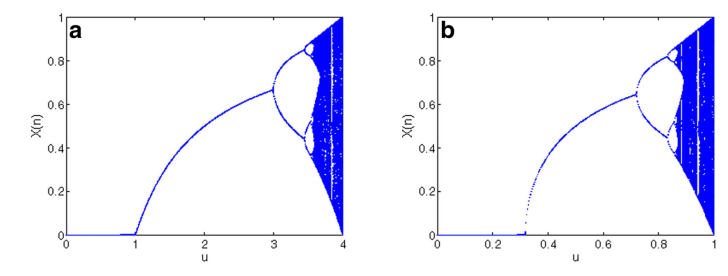
\includegraphics[scale=0.7]{graphics/chapter-1/chap1-logistic_sine_map.png}
    \caption{Logistic map (a) và sine map (b)}
    \label{fig:chap1-logistic_sine_map}
\end{figure}

\subsection{Improved 1D chaotic system model}

Hàm 1D chaotic được cải tiến được thể hiện như sau:

\begin{equation}
\label{eq:improved-1d-chaotic}
\begin{multlined}
f_{ic}(u,x_{n+1},k) = mod(f_c(u,x_n) \times g(k),1). \\
where g(k) = 2^k, 9 \leq k \leq 16.
\end{multlined}
\end{equation}

Tham số hệ thống $u$ vẫn nằm trong đoạn $(0,4]$ và có thể mở rộng thêm. $f_c(u,x_n)$ là hàm 1D chaotic map hiện tại, $f_{ic}(u,x_{n+1},k)$ là hàm đã được cải tiến của mô hình đề xuất. $k=12$ là giá trị tốt nhất (sau khi đã thực nghiệm).

\subsection{Improved 1D chaotic map and performance evaluation}

Dựa trên những cải tiến của hàm chaotic tại \ref{eq:improved-1d-chaotic}, hàm logistic map được thể hiện như sau:
\begin{equation}
\label{eq:improved_logistic_map}
x_{n+1} = mod(u \times x_n \times (1 - x_n ) \times 2^{12}, 1)
\end{equation}
và hàm sine map được cải tiến như sau:
\begin{equation}
\label{eq:improved_sine_map}
x_{n+1} = mod( u \times \sin(\pi \times x_n) \times 2^{12},1)
\end{equation}

\textbf{Hình \ref{fig:chap1-improved_map}} mô tả phân bố của các hàm logistic và sine sau khi cải tiến hàm chaotic.

\begin{figure}
    \centering
    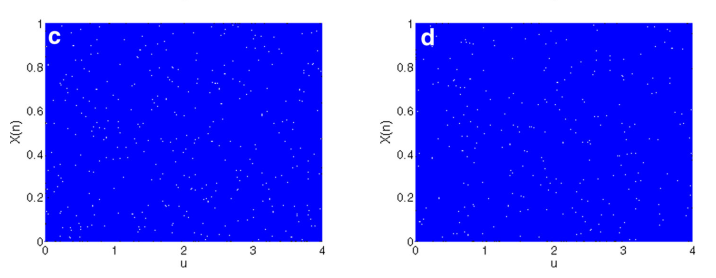
\includegraphics[scale=0.7]{graphics/chapter-1/chap1-improved_map.png}
    \caption{Distribubtions của hai hàm logisctic map (c) và sine map}
    \label{fig:chap1-improved_map}
\end{figure}

Số mũ Lyapunov là một chỉ số để đánh giá  hiệu suất của chaotic map và có các đặc tính hỗn loạn tốt khi giá trị lớn hơn 0. Số mũ Lyapunov của chaotic map hiện tại và của phiên bản cải thiện được thể hiện trong \textbf{Hình \ref{fig:chap1-lyapunov}}. 



\begin{figure}
    \centering
    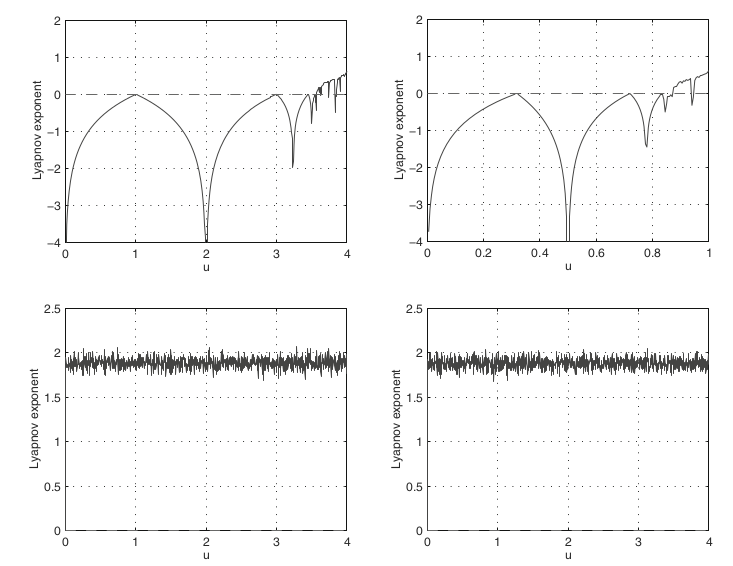
\includegraphics[scale=0.7]{graphics/chapter-1/chap1-lyapunov.png}
    \caption{Biểu đồ số mũ Lyapunov logistic map (a), sine map (b) và phiên bản cải tiến của nó}
    \label{fig:chap1-lyapunov}
\end{figure}

Ngoài ra, entropy là chỉ số đánh giá hiệu suất của chaotic map, là một chỉ số để đánh giá sự không ổn định của các giá trị ngẫu nhiên, có nghĩa là nó có tối đa giá trị khi tất cả các tín hiệu được phân phối ngẫu nhiên và giá trị càng gần với 8 thì đặc tính phân phối càng tốt.
Hàm entropy, được thể hiện trong công thức sau
\begin{equation}
\label{eq:entropy}
I(R) = \sum_{i=0}^{F - 1 } P(R=i) \times \log_2P(R = i)
\end{equation}
trong đó $P$ là hàm mật độ xác suất rời rạc. \textbf{Hình \ref{fig:chap1-entropy}} cho thấy sự tương phản giữa chỉ số entropy chaotic map hiện có và phiên bản được cải tiến. Nó cho thấy rằng chaotic map được cải thiện có các đặc điểm phân phối hoàn toàn vượt trội. Các kết quả thử nghiệm này cho thấy mô hình hệ 1D chaotic system được đề xuất là rất chính xác.

\begin{figure}
    \centering
    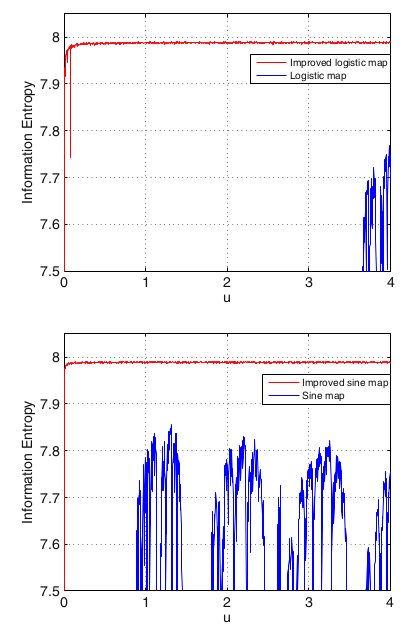
\includegraphics[scale=0.5]{graphics/chapter-1/chap1-entropy.png}
    \caption{Chỉ số entropy của hàm hiện tại (a) và bản cải ttiến}
    \label{fig:chap1-entropy}
\end{figure}

\section{Proposed LSB steganography algorithm}
\subsection{Embedding process}

Quá trình nhúng là một quá trình ẩn dữ liệu bí mật trong ảnh bìa và các tệp hình ảnh và văn bản có thể được sử dụng làm dữ liệu bí mật. Thuật toán như sau.

\begin{itemize}
    \item \textbf{Bước 1}: Đọc ảnh bìa và dữ liệu bí mật.
    Đọc ảnh bìa và lấy giá trị pixel trung bình của ảnh bìa theo phương trình sau
    \begin{equation}
    \label{eq:read_cover_secret}
    PM_c = \sum_{k=1}^c \sum_{i=1}^M \sum_{j=1}^n cp_{ij} \mathbin{/} (c \times M \times N)
    \end{equation}
    với $c=3$ là giá trị của bảng màu RGB, $M$ và $N$ là chiều cao và chiều rộng của ảnh bìa và $cp_{ij}$ là giá trị pixel của ảnh bìa. 
    Tiếp theo, dữ liệu bí mật được nhúng được đọc và chuyển đổi thành ma trận một chiều và giá trị trung bình của dữ liệu bí mật thu được theo phương trình sau.
    \begin{equation}
    \label{eq:secret_data}
    PM_s = \sum_{i=1}^{sLen} sd_i \mathbin{/} sLen
    \end{equation}
    với $sd_i$ là giá trị phần tử ma trận một chiều của dữ liệu bí mật và sLen là độ dài dữ liệu bí mật.
    \item \textbf{Bước 2:} Xác định các tham số ban đầu của chaotic map và tạo khóa.
    Từ giá trị $PM_c$ và $PM_s$ được tính tại \textbf{Bước 1}, các tham số ban đầu của chaotic map được tính toán như sau.
    \begin{equation}
    \label{eq:chaotic_x0}
    x'_0 = x_0 \times PM_c - floor(x_0 \times PM_c)
    \end{equation}
    \begin{equation}
    \label{eq:chaotic_u}
   u' = 4 \times (u \times PM_s - floor(u \times PM_s))
    \end{equation}
    với $u' \in [0,4], x'_0 \in [0,1]$
    Bằng cách đặt $x'_0$ và $u'$ được tính toán lại làm tham số hệ thống ban đầu của 1D chaotic map bản cải tiến, chúng ta có thể rút ra chuỗi $XM = \{x_1, x_2,...x-s \}$ có kích thước $s$ được tính theo phương trình \ref{eq:s_size_output} và $bc_{lsb}=4$ là số bit LSB của ảnh bìa.
    \begin{equation}
    \label{eq:s_size_output}
    s = (c \times M \times N \times bc_{lsb})
    \end{equation}
    \item \textbf{Bước 3:}Tính toán ma trận vị trí nhúng.
    Chúng ta có ma trận vị trí $P = \{p_1, p_2,...p_s \}$ bằng cách sắp xếp đầu ra của chaotic map $XM$ theo quy trình tại \textbf{Hình \ref{fig:chap1-position-matrix-generate}}
    Từ ma trận vị trí $P$, chúng ta tính toán được ma trận nhúng $EP = \{ep_1, ep_2,...ep_s \}$ với $ep_i = \{ p_{cp}(i), p_{row}(i), p_{col}(i)\}$ được tính theo các phương trình \ref{eq:embed_pcp}, \ref{eq:embed_prow}, \ref{eq:embed_pcol}
    \begin{equation}
    \label{eq:embed_pcp}
    p_{cp}(i) = floor((p(i) - 1) \mathbin{/}(M \times N)) + 1
    \end{equation}
    \begin{equation}
    \label{eq:embed_prow}
    p_{row}(i) = mod((p(i) -1), N) +1
    \end{equation}
    \begin{equation}
    \label{eq:embed_pcol}
    p_{col}(i) = mod((floor((p(i) -1) \mathbin{/} M),N) +1
    \end{equation}
    với $ 1 \leq p_{cp}(i) \leq c, 1 \leq p_{row}(i) \leq M, 1 \leq p_{col}(i) \leq N.$
    $p_{cp}(i)$là số bảng màu của vị trí nhúng dữ liệu bí mật, $p_{row}(i)$ là vị trí hàng được nhúng và $p_{col}(i)$ là vị trí cột.
    Phương trình \ref{eq:embed_pcp} - \ref{eq:embed_pcol} được tính toán lặp đi lặp lại theo $s$ lần và ma trận vị trí nhúng thu được cung cấp tất cả thông tin về các vị trí nhúng dữ liệu bí mật.
    \item \textbf{Bước 4}: Quy trình nhúng
    Đầu tiên tạo ma trận bit một chiều $sb = \{sb_1, sb_2,...sb_{sLen}\}$ của dữ liệu bí mật. Theo ma trận $EP$ được tính toán tại \textbf{Bước 3}, bốn bit của $sb$ ma trận sẽ được nhúng trong các bit LSB của ảnh bìa dưới dạng một đơn vị và quá trình này có thể được biểu diễn như sau.
    \begin{equation}
    \label{eq:embeđe_process}
    cp_{lsb}(p_{cp}(i), p_{row}(i), p_{col}(i)) = sb(i \times 4 -3 : i \times 4)
    \end{equation}
    với $1 \leq i \leq (2 \times sLen)$ và $cp_{lsb}$ là bit LSB của ảnh bìa.
\end{itemize}
\textbf{Bước 4} thực hiện $(2 \times sLen)$ lần tới chừng nào hình ảnh stego hoàn thành. Trong trường hợp dữ liệu bí mật được nhúng là một hình ảnh, cần phải chuyển đổi dữ liệu hình ảnh bí mật sang ma trận một chiều ở \textbf{Bước 1}
\begin{figure}
    \centering
    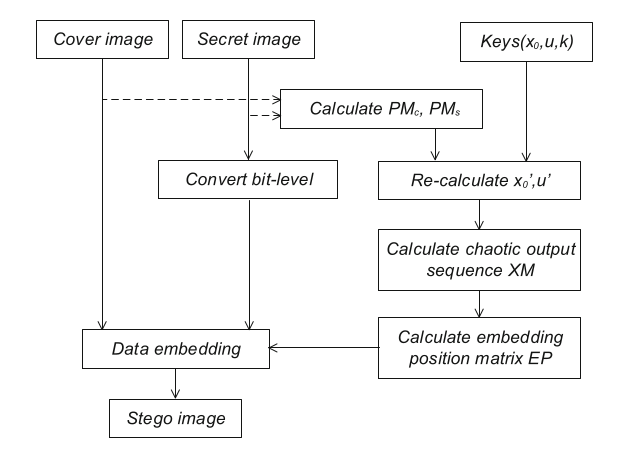
\includegraphics[scale=0.6]{graphics/chapter-1/chap1-proposed_algorithm.png}
    \caption{Lưu đồ tổng thể thuật toán đề xuất}
    \label{fig:enter-label}
\end{figure}

\begin{figure}
    \centering
    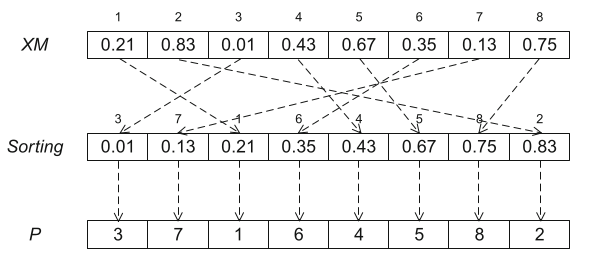
\includegraphics[scale=0.6]{graphics/chapter-1/chap1-position-matrix-generate.png}
    \caption{Sơ đồ sinh ma trận vị trí}
    \label{fig:chap1-position-matrix-generate}
\end{figure}

\subsection{Extracting process}
Ở giai đoạn này, trích xuất dữ liệu bí mật được chèn vào hình ảnh stego và nó có thể được coi là quá trình ngược lại với quy trình nhúng. $(x_0, u_0, k, PM_c, PM_s, sLen)$ là các khóa bí mật và quá trình trích xuất có thể được biểu diễn như sau.
\begin{equation}
\label{eq:extract_process}
sb(i \times 4 - 3 : i \times 4) = cp_{lsb}(p_{cp}(i), p_{row}(i), p_{col}(i))
\end{equation}
với $1 \leq i \leq (2 \times sLen)$. Ma trận bit thu được bằng cách lặp lại $(s \times sLen)$ lần được chuyển thành ma trận byte. Do đó, thông tin bí mật ban đầu thu được.
Trường hợp dữ liệu bí mật được nhúng là ảnh thì cần chuyển ma trận một chiều thu được thành ma trận hai chiều tương ứng với kích thước của ảnh mật.
\chapter{Cơ sở lý thuyết và các nghiên cứu liên quan}
\label{chapter2}

% Print references
\fancyhf{}
\printbibliography[heading=bibintoc, title = {Tài liệu tham khảo}]
\end{document}
